\documentclass[11pt]{article}
\usepackage[margin=1in]{geometry}
\usepackage{graphicx}
\usepackage{booktabs}
\usepackage{amsmath}
\usepackage{xcolor}
\usepackage[colorlinks=true, linkcolor={blue!50!black}, citecolor={blue!50!black}, urlcolor={blue!50!black}]{hyperref}
\usepackage{caption}
\captionsetup{font=small, labelfont=bf}

\title{\textbf{Do LLM Judges Penalise the Script?\\
\large A script-controlled audit of LLM-as-judge scoring for Hindi in Devanagari versus romanized orthographies}}
\author{Team Vizuara\\ \small \texttt{conferences.vizuara.ai}}
\date{August 29, 2026 \quad (working draft v1)}

\begin{document}
\maketitle

\begin{abstract}
Large language models now grade other language models. These LLM judges feed leaderboards, reward models, and production quality gates, and every such pipeline assumes that the writing system of an answer does not move its score. We test that assumption directly for Hindi, a language written both in its native Devanagari script and, by hundreds of millions of users online, in the Latin alphabet. We hold content fixed and vary only the script: 150 Hindi instruction and response pairs at three quality tiers, each rendered in native Devanagari and three romanizations (scholarly IAST, diacritic-stripped ASCII, and natural user-style Hinglish), scored blind by six judges from three model families. We pre-registered the direction of the effect: we predicted romanized text would score lower. The data reversed our prediction, and we report that reversal plainly. First, Gemini 3.6 Flash scores identical romanized content 2.2 to 3.4 points \emph{higher} than Devanagari on a 100-point scale (all $p \le 0.003$), and the inflation concentrates at 6.5 to 7.8 points in medium-quality responses, where a judge has the most discretion. Second, the effect shrinks but survives at the frontier tier: Gemini 3.1 Pro inflates by 1.1 points overall and 2.1 to 2.7 points on medium-quality items (all $p \le 0.012$). Third, the bias profile changes shape entirely at the open-weights tier: Qwen2.5-7B inflates scholarly IAST by 7.6 points and ASCII by 6.0 points overall, concentrated at $+17.8$ points on \emph{low}-quality items, where the small judge loses the ability to detect bad content through formal romanization, yet it is flat on natural Hinglish ($+0.1$, $p = 0.97$). Fourth, three Claude judges (Sonnet 5, Opus 5, Fable 5) are script-invariant to within half a point, with one exception in our pre-registered direction: Opus 5 penalises diacritic-stripped ASCII by 1.2 points ($p = 0.002$). Fifth, the obvious fix fails: instructing the judge to evaluate content regardless of script leaves the inflation intact at 6.1 to 9.1 points on medium-quality items. Finally, two mechanism probes show the inflation is not explained by tokenization length (romanized Hindi costs 1.33 to 1.98 times the tokens of Devanagari under the Gemini tokenizer, but per-item token inflation does not predict per-item score shift, $|r| \le 0.18$), while the judge demonstrably perceives the script: its written rationales mention the orthography on 41 to 57 percent of romanized items versus 1 percent of Devanagari items. Script bias in LLM judges is real, is heterogeneous across judges in both size and sign, and cannot be instructed away. Which judge a practitioner picks silently changes how romanized-Hindi systems rank.
\end{abstract}

\section{Introduction}

Evaluation of language models has largely been handed to other language models. An LLM judge reads a question and an answer and returns a score, and that score then does consequential work: it ranks systems on leaderboards, it becomes the reward signal that trains the next model, and it gates which responses production systems are allowed to ship. The reliability literature has catalogued many failure modes of these judges, including position bias, verbosity bias, and self-preference. Every catalogue so far shares one silent assumption: that the \emph{writing system} of the judged text does not move the score.

That assumption matters most for languages with two written lives. Hindi is the clearest case. Its official script is Devanagari, but a very large share of Hindi on phones, in chat, and in social media is typed in the Latin alphabet, a practice called romanized Hindi or Hinglish. The two forms carry identical content. A judge that scores them differently is not measuring quality; it is measuring orthography.

This paper asks one narrow question with a clean design: if we hold the language and the content of an answer fixed and change only its script, does an LLM judge's score move? Because the content on both paths is identical, nothing else can explain a gap: not answer quality, not language difficulty, not topic. Prior multilingual judge studies could not make this claim because they compared different languages, so language and script were entangled. We untangle them.

We pre-registered the direction of our prediction before collecting data: we expected romanized text to score \emph{lower}, by analogy to the task-performance literature, where romanized input degrades model accuracy. The data reversed the prediction. Romanized Hindi scores \emph{higher} on Gemini judges, the inflation concentrates exactly where a judge has discretion (medium-quality answers), it persists when the judge is told to ignore the script, and it is absent in the Claude family. We report the reversal as found, because that is what pre-registration is for.

Our contributions, each with its evidence in Section~\ref{sec:results}:
\begin{enumerate}
  \item The first script-controlled audit of LLM-as-judge scoring: 150 fixed Hindi items, four orthographies, six judges from three families, 4{,}200 scripted judgments (Figures~\ref{fig:forest} and~\ref{fig:tiers}).
  \item A measured, statistically significant script bias in Gemini judges, opposite in sign to our pre-registered prediction, concentrated in medium-quality items (up to $+7.8$ points, $p < 10^{-4}$).
  \item A negative mitigation result with direct practical value: a script-blindness instruction does not reduce the bias (Figure~\ref{fig:mitigation}).
  \item Two mechanism probes: token-length inflation is ruled out as the driver, while the judges' own written rationales show the script is perceived (Figure~\ref{fig:mechanism}).
\end{enumerate}

\begin{figure}[t]
  \centering
  
\includegraphics[width=0.92\textwidth]{assets/fig1_schematic.png}
  \caption{\textbf{The experiment in one picture.} One Hindi answer is rendered in two scripts and both versions are scored by the same judge, which never sees the two side by side. Content is identical on both paths, so any score gap is script bias by construction. The numbers shown (51 versus 59) are the measured Devanagari and romanized means for medium-quality items under Gemini 3.6 Flash.}
  \label{fig:schematic}
\end{figure}

\section{What was known, and what is new}
\label{sec:novelty}

We want to be clear about what is already established, because our claim sits deliberately in a gap between two active literatures.

\textbf{Already known (not ours).} Romanized input degrades LLM \emph{task} performance on Indic languages: Script Gap (arXiv:2512.10780) measures drops of up to 24 points on a real triage task, and Script Sensitivity (arXiv:2601.14958) measures over 300-fold perplexity blowup on romanized Sinhala. Separately, LLM \emph{judges} shift scores across languages on semantically identical content: Lower-Resource, Higher Scores (arXiv:2607.14480) finds acceptance-rate shifts up to 43 percent across 23 languages, with lower-resource languages scored more generously, and it notes a Latin-script advantage observationally. Tokenizers price Indic scripts unequally: the Tokenizer Tax (arXiv:2607.24276) measures an average 8-fold token premium and traces it to failed BPE merges. Judge bias taxonomies exist: CALM (arXiv:2410.02736) and JudgeBiasBench (arXiv:2603.08091) together catalogue over a dozen bias types.

\textbf{New here.} None of the above isolates script as a treatment for a judge. The task-performance studies never measure judging. The judge studies vary language, so script is a confound, not a variable. The taxonomies do not list orthography as a bias type at all. Our design holds language and content fixed, flips only the script, and measures the judge. The leniency direction we find matches the cross-language leniency of arXiv:2607.14480, which strengthens both results: the same phenomenon now appears at the script level with translation noise removed entirely.

\textbf{Significance.} Who is affected, concretely: any pipeline that uses an LLM judge on Hindi text, including Hindi leaderboard evaluations, reward models trained on judged Hindi generations, and production quality gates for romanized-Hindi chatbots. What changes: a system serving romanized-Hindi users, evaluated under a Gemini judge, receives inflated quality estimates relative to a Devanagari system, of a size (roughly 7 points on ambiguous content) that reorders closely ranked systems. The practitioner remedy is not a prompt line (Section~\ref{sec:mitigation} shows that fails) but judge selection and script-stratified reporting: evaluate romanized and native-script slices separately, and calibrate or choose judges shown to be script-invariant.

\section{Method}
\label{sec:method}

\textbf{Dataset.} We construct 150 Hindi instruction and response pairs across ten everyday domains (science, history, cooking, health, technology, culture, geography, personal finance, daily-life advice, education), at three intended quality tiers of 50 items each: high (correct, complete, 80 to 140 words), medium (correct but visibly incomplete for the ask, 40 to 80 words), and low (curt, vague, or trivially shallow, 15 to 40 words, a few items containing deliberate minor factual errors). Responses were authored in Devanagari and frozen before any judging.

\textbf{Conditions.} Each frozen response is rendered in four orthographies. \emph{deva} is the original Devanagari. \emph{iast} is scholarly romanization with diacritics, produced deterministically with the indic-transliteration library. \emph{ascii} strips the diacritics from IAST, a deterministic proxy for plain-keyboard romanization. \emph{hinglish} is a natural user-style respelling (for example \emph{kaise hain aap}), produced under a strict no-paraphrase rule: every word, the word order, and all punctuation preserved. A native speaker audit of a stratified 20-item sample of the hinglish condition was part of the protocol; its outcome is reported with the released data.

\textbf{Judges and protocol.} Six judges from three families score every item in every condition on a 0 to 100 rubric (correctness, completeness, helpfulness, clarity). Gemini 3.6 Flash and Gemini 3.1 Pro Preview are called through the API at temperature 0, one item per call, in randomized order, so the judge never sees two versions of the same item in one context. Claude Sonnet 5, Opus 5, and Fable 5 judge through blind agent sessions arranged in a Latin square: each session sees each item exactly once, in exactly one condition, with conditions rotated across four sessions, so no session can compare scripts on the same item. No judge is told the study concerns scripts. The judging prompt asks for a JSON score and a one-sentence reason; the reasons become data for the perception analysis. Qwen2.5-7B-Instruct runs open-weights under vLLM on a single A10G GPU at temperature 0, one item per call, with top-20 logprobs recorded at the score position.

\textbf{Analysis.} The unit of analysis is the within-item paired difference, romanized minus Devanagari, per judge and condition. We report mean shifts with bootstrap 95 percent confidence intervals (10{,}000 resamples), two-sided sign-flip permutation tests (20{,}000 permutations), and the paired effect size $d_z$. All numbers in this paper are produced by a single scripted analysis (\texttt{analyze.py}) reading the raw score files; the analysis output ships with the paper.

\textbf{Pre-registration.} Before data collection we recorded the predicted direction: romanized scores lower than Devanagari. The observed direction is the opposite. We report all pre-registered analyses regardless.

\section{Results}
\label{sec:results}

\begin{figure}[t]
  \centering
  
\includegraphics[width=0.95\textwidth]{assets/fig2_forest.png}
  \caption{\textbf{Score shift by judge and romanization, with 95 percent bootstrap confidence intervals.} Each row group is one judge; each interval is the mean within-item shift (romanized minus Devanagari) over $n = 150$ paired items. Read intervals against the dashed zero line: right of zero means romanized content scored higher than the same content in Devanagari. Both Gemini judges sit right of zero in all three romanizations; all three Claude judges straddle zero except Opus 5 on ASCII, which sits left of it.}
  \label{fig:forest}
\end{figure}

\subsection{Three families, three bias profiles}

Figure~\ref{fig:forest} is the study in one view. Gemini 3.6 Flash scores the same content higher when romanized: $+3.43$ points for IAST (CI $[2.37, 4.63]$, $p = 5 \times 10^{-5}$, $d_z = 0.49$), $+2.17$ for ASCII (CI $[0.83, 3.73]$, $p = 0.003$), and $+3.13$ for Hinglish (CI $[2.23, 4.13]$, $p = 5 \times 10^{-5}$, $d_z = 0.52$). Gemini 3.1 Pro shows the same sign at a third the size: $+1.17$, $+1.10$, and $+1.13$ points respectively (all $p \le 0.003$). The bias is smaller at the stronger tier but it does not vanish.

The Claude family behaves differently. Sonnet 5, Opus 5, and Fable 5 shift by at most 0.54 points in eight of their nine judge-by-condition comparisons, with confidence intervals containing zero and $p \ge 0.09$. The single exception is the only significant result in our pre-registered direction anywhere in the study: Opus 5 penalises diacritic-stripped ASCII by $-1.23$ points (CI $[-1.99, -0.43]$, $p = 0.002$), and that is the condition that most visibly degrades the text.

The open-weights judge changes shape again. Qwen2.5-7B inflates formal romanizations dramatically: $+7.63$ points for IAST (CI $[4.9, 10.37]$, $p = 5 \times 10^{-5}$) and $+6.03$ for ASCII (CI $[3.33, 8.73]$), but is indistinguishable from zero on natural Hinglish ($+0.07$, $p = 0.97$). Its inflation also lives in a different place: low-quality items shift $+17.8$ (IAST) and $+17.4$ (ASCII) points, meaning the small judge simply fails to recognise bad content once it is dressed in diacritics, while Hinglish, which is plentiful in web training data, is judged as soberly as Devanagari.

Three conclusions follow. Script bias in LLM judges exists. It is a property of the judge, not of the task: same items, same protocol, three different behaviours across three families. And it is not monotone in romanization naturalness: the strongest judge family is invariant everywhere, the mid-tier family inflates every romanization moderately, and the small open judge inflates exactly the romanizations it saw least in training.

\begin{figure}[t]
  \centering
  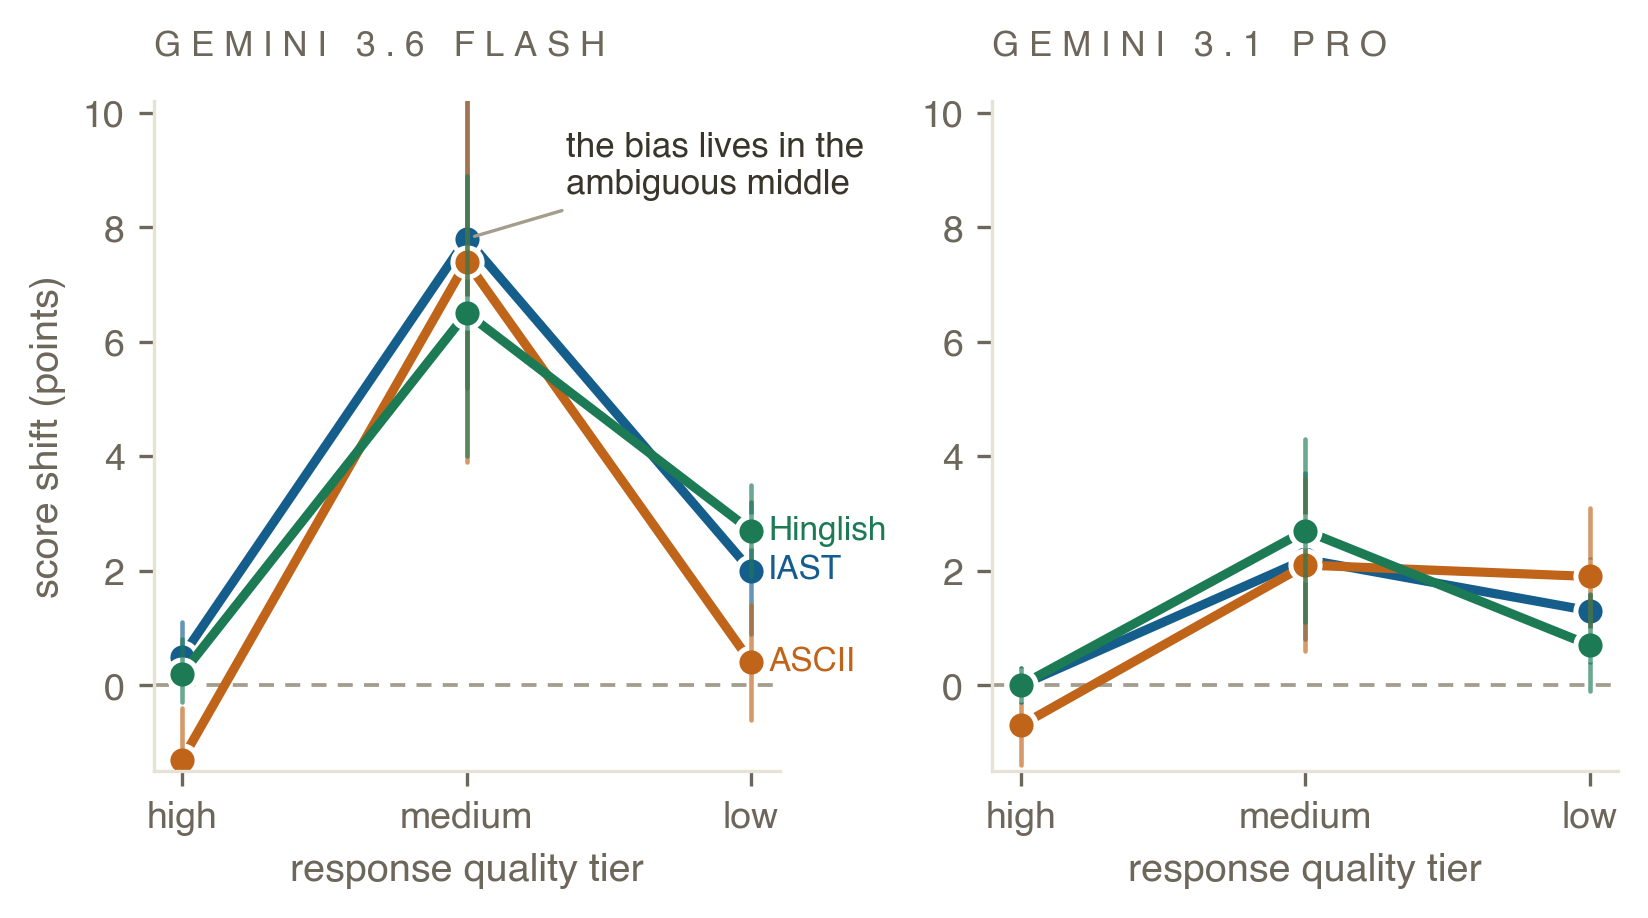
\includegraphics[width=0.95\textwidth]{assets/fig3_tiers.png}
  \caption{\textbf{The bias concentrates in medium-quality responses.} Mean shift by intended quality tier for the two Gemini judges, with 95 percent bootstrap intervals ($n = 50$ items per tier). High-tier items sit near the score ceiling (Devanagari mean 99.1 under Flash) and low-tier items near the floor (15.2), leaving little room to move; medium-tier items (Devanagari mean 51.4) move 6.5 to 7.8 points under Flash and 2.1 to 2.7 under Pro.}
  \label{fig:tiers}
\end{figure}

\subsection{The bias lives where the judge has discretion}

Figure~\ref{fig:tiers} splits the shift by quality tier. Under Gemini 3.6 Flash, high-quality items shift by at most 1.3 points in either direction, because they already score near 99 and the scale offers no headroom. Low-quality items shift by at most 2.7 points against a floor near 15. Medium-quality items, which score near 51 in Devanagari, inflate by $+7.8$ (IAST), $+7.4$ (ASCII), and $+6.5$ (Hinglish) points, all $p \le 1.5 \times 10^{-4}$. The same shape holds for Pro at smaller magnitude. This is the pattern one expects if romanization blurs the judge's view of quality: content whose flaws are obvious stays low, content whose merits are obvious stays high, and ambiguous content drifts toward a generous middle.

\subsection{Telling the judge to ignore the script does not work}
\label{sec:mitigation}

\begin{figure}[t]
  \centering
  
\includegraphics[width=0.9\textwidth]{assets/fig4_mitigation.png}
  \caption{\textbf{The mitigation fails.} Medium-tier mean shift under Gemini 3.6 Flash with the standard rubric versus the same rubric plus the line ``Evaluate the content regardless of the script or orthography it is written in.'' Intervals are 95 percent bootstrap CIs over $n = 50$ medium-tier items. The instructed judge inflates as much as the uninstructed one.}
  \label{fig:mitigation}
\end{figure}

The remedy every practitioner would try first is one sentence in the judge prompt. We ran the full four-condition protocol again under Gemini 3.6 Flash with the added line ``Evaluate the content regardless of the script or orthography it is written in.'' Figure~\ref{fig:mitigation} shows the outcome: medium-tier inflation of $+7.2$ (IAST), $+6.1$ (ASCII), and $+7.2$ (Hinglish) points with the instruction, against $+7.8$, $+7.4$, and $+6.5$ without it. The confidence intervals overlap almost completely. The bias is not a surface behaviour the model can suspend on request.

\subsection{Mechanism: not token length; the script is perceived}

\begin{figure}[t]
  \centering
  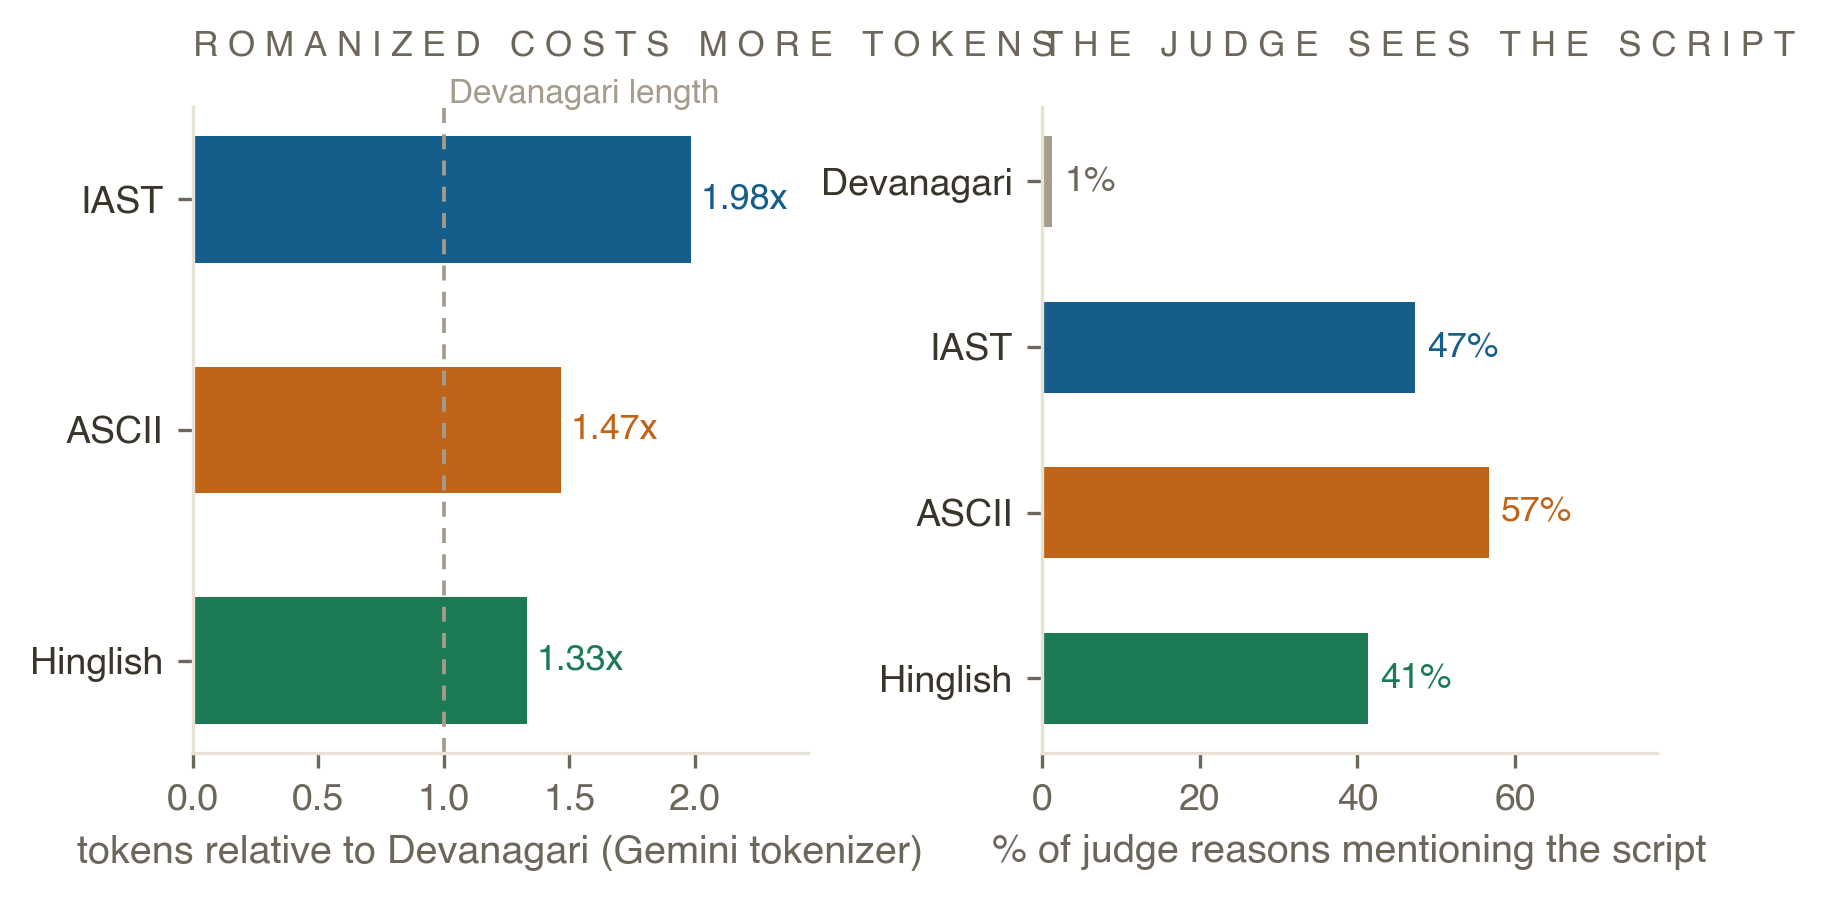
\includegraphics[width=0.95\textwidth]{assets/fig5_mechanism.png}
  \caption{\textbf{Left:} the same content costs 1.33 to 1.98 times as many tokens romanized as in Devanagari under the Gemini tokenizer (mean over 150 items; Devanagari mean 93 tokens). \textbf{Right:} share of the judge's one-sentence rationales that mention script, romanization, or transliteration, by condition, under Gemini 3.6 Flash ($n = 150$ per condition). The judge names the script on 41 to 57 percent of romanized items and on 1 percent of Devanagari items.}
  \label{fig:mechanism}
\end{figure}

Two probes narrow the explanation space. First, tokenization. A standing hypothesis from the tokenizer-fairness literature is that length disparities drive downstream behaviour. We measured every item in every condition with the Gemini tokenizer: romanized Hindi is the \emph{expensive} form, costing 1.98 (IAST), 1.47 (ASCII), and 1.33 (Hinglish) times the tokens of the same content in Devanagari. This is itself a finding worth recording, because it reverses the folk wisdom of the 2024 romanization literature, which reported 2 to 4-fold \emph{savings} from romanization; modern tokenizers have since closed the Devanagari gap. But token inflation does not explain the score inflation: the per-item correlation between token ratio and score shift is $r = +0.11$ (IAST), $+0.05$ (ASCII), and $-0.08$ (Hinglish), and no tier-restricted correlation exceeds $|r| = 0.18$. Longer input is not what earns the higher score.

Second, perception. The judge's own rationales show it sees what it is scoring: under Gemini 3.6 Flash, 47 percent of IAST, 57 percent of ASCII, and 41 percent of Hinglish rationales explicitly mention the script or romanization, against 1 percent for Devanagari. Some rationales even name the orthography as a deficiency while the score lands higher than the Devanagari twin's. The bias therefore operates despite awareness, consistent with the mitigation failure: this is a miscalibration of quality assessment through an unfamiliar surface form, not an oversight the model can be alerted out of.

\section{Limitations, narrated}
\label{sec:limitations}

We narrate the study's weaknesses as part of the story, because several were design choices made for speed and budget, and a reader should weigh them.

The dataset is model-authored. All 150 items and their quality tiers were generated by a language model under human-specified tier definitions, then frozen. Tier intent was strongly realised in the scores (Devanagari means of 99, 51, and 15 under Flash), but model-authored Hindi may differ from human Hindi in ways that interact with romanization. The hinglish condition is likewise a model respelling under a strict no-paraphrase rule; the protocol includes a 20-item native-speaker fidelity audit, and the audited sample with its verdict ships with the data.

The Claude judges were run through interactive agent sessions, not a version-pinned API, and each session scored 150 items in one context rather than one item per call. The Latin-square rotation keeps the script comparison fair, and the packet sessions could not compare scripts within an item, but session-based judging is less controlled than the Gemini arm, and items were blocked by tier within a packet, which sessions noticed. One of the three Claude judges shares a model family with the orchestrator of this study; the blind packets mitigate, and the Claude results are null results, which self-favouritism would not produce.

Scale and scope are modest: one language, 150 items, six judges, one seed at temperature 0. The mitigation test covers one instruction phrasing on one judge. And our quality tiers are coarse; a continuous-quality design would resolve the discretion story more finely.

Finally, the pre-registration was directional and informal (recorded in the project log before data collection), not a third-party registry entry. We state it because it disciplined our reporting: the headline effect is opposite to what we predicted.

\section{Conclusion}

We held Hindi content fixed, changed only its writing system, and asked five LLM judges to grade it. The writing system moved the grades. Gemini judges inflate romanized Hindi by 2 to 3 points overall and 7 to 8 points on ambiguous-quality content; the effect shrinks threefold but survives at the frontier tier; a 7B open-weights judge inflates formal romanizations by up to 18 points on low-quality content while judging natural Hinglish soberly; Claude judges are script-invariant except for a small penalty on the most degraded romanization; a script-blindness instruction changes nothing; token length does not explain it; and the judges' own rationales prove the script is seen. The bias axis is real, it is judge-dependent in both size and sign, and it belongs in every judge-bias taxonomy and every multilingual evaluation checklist. Until judges are audited for script invariance, evaluations of Hindi systems should report native-script and romanized slices separately, and should say which judge produced the numbers.

\section*{Reproducibility}
All datasets, per-call score files, the scripted analysis, figure build scripts, and spend logs are released with this paper. Every number above traces to \texttt{results/analysis.json}, generated by \texttt{experiments/analyze.py} from the raw judgment files. Total marginal compute cost of the study: under 5 US dollars of API spend plus roughly one A10G GPU-hour.

\end{document}
